\documentclass[10pt,a4paper]{article}


\usepackage[utf8]{inputenc}
\usepackage[spanish,english, es-tabla, es-noshorthands]{babel}


\captionsetup[figure]{font=footnotesize}
\usepackage{siunitx}
\usepackage{amsmath}
\usepackage{amsfonts}
\usepackage{amssymb}
\usepackage{float}
\usepackage{textcomp}
\usepackage{siunitx}
\usepackage{graphicx, wrapfig}
\usepackage{caption}
\usepackage{subfig}
%\usepackage{subcaption}
\usepackage{multicol}
\usepackage{multirow}

\title{PLL}


\begin{document}
\section{PLL: Phase Locked Loop}

\subsection{Introducción}

Un lazo de seguimiento de fase, o phase locked loop, es un sistema de control que genera una señal en su salida cuya fase está relacionada con la fase de la señal en su entrada. En el presente informe, se implementa un PLL mediante el uso de un circuito integrado de bajo consumo, el CD4046B, que consta de un oscilador controlado por voltaje (VCO, por sus siglas en inglés), dos comparadores de fase y un filtro pasa-bajos. Se buscara saber acerca de su funcionamiento y cuales sus limites mientras opera. 
Se preparó el CD4046 con un setup recomendado por la catedra que se muestra en la figura \ref{Circuito PLL}. Teniendo en cuenta que no se puede colocar una señal negativa en la entrada se procedio a trabajar sobre el circuito armado.

\begin{figure}
	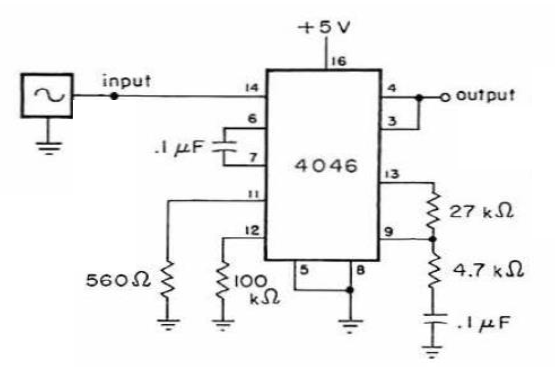
\includegraphics[scale=1]{..\PLL\Imagenes\Circuito PLL.png}
	\centering
	\label{Circuito PLL}
	\caption{Setup recomendado}
\end{figure}

\subsection{Transferencia}




\end{document}